\chapter{Electrical measurements}
\label{sec:Experiment}

    This chapter describes the experimental setup, and presents the results of the measurements taken.
    
\section{Measurement setup} \label{sec:ExperimentMeasurementSetup}

    In order to characterise a single storage element, as well as examine the behaviour of series connections, the experimental equipment should be able to:
    \begin{itemize}[noitemsep,label=\textbullet]
    	\item Apply and measure external magnetic field perpendicular to the sample plane.
    	\item Measure the resistance of the sample
    	\item Apply short (\textasciitilde\SI{1}{\milli\second}) square voltage pulses and measure the resistance during each pulse.
    	\item Provide precise and stable connection to the sample contact pads
    \end{itemize}
    
    All the requirements were met by using the setup presented in Figs. \ref{ExperimentMeasurementSetup} and \ref{ExperimentMeasurementPhoto}. The equipment used for the experiment consists of:
    
    \begin{itemize}[noitemsep,label=\textbullet]
    	\item GMW Dipole Electromagnet, model 3470, capable of generating magnetic field up to \SI[per-mode=symbol]{790}{\kilo\ampere\per\metre}
    	\item Kepco BOP-series power supply (voltage controlled current source) with digital-to-analog USB adapter
    	\item LakeShore 475 DSP Gaussmeter with Hall probe
    	\item Keithley 2636A Sourcemeter
    	\item Set of micropositioners equipped with tungsten or gold tips of ca.  \SI[parse-numbers = false, number-math-rm = \ensuremath]{20-50}{\micro\metre} in diameter
    	\item PC with LabVIEW software for measurement automation
    	\item microscope for positioning of the test tips
    \end{itemize}
    
    \begin{figure}[H]
        \centering
        \includegraphics[width=0.65\paperwidth, page=1]{img/05/MeasurementSetup.pdf}
        \caption{The schematic drawing of the measurement station. (1) denotes sample, (2) tungsten or gold tips, (3) Hall probe, (4) micropositioners.}
        \label{ExperimentMeasurementSetup}
    \end{figure}
    
\begin{figure}[H]
    \centering
    \begin{subfigure}[t]{0.35\paperwidth}
    	\centering
    	\vskip 0pt
        \includegraphics[width=0.3\paperwidth]{img/05/SetupPhoto2.jpg}
        \caption{Photo of the main part of the measurement setup, including micropositioners, Hall probe and electromagnet. The mirror and the microscope is used to watch the sample while connecting the tips.}
        \label{ExperimentMeasurementPhotoa}
    \end{subfigure}
    ~ %add desired spacing between images, e. g. ~, \quad, \qquad, \hfill etc. 
      %(or a blank line to force the subfigure onto a new line)
    \begin{subfigure}[t]{0.35\paperwidth}
    	\centering
    	\vskip 0pt
        \includegraphics[width=0.3\paperwidth]{img/05/SetupPhotoMicro.jpg}
        \caption{Microscopic image of the sample under measurement with tungsten tips connected.}
        \label{ExperimentMeasurementPhotob}
    \end{subfigure}
    \caption{Photos of the measurement setup.}
    \label{ExperimentMeasurementPhoto}
\end{figure}

\subsection{Measurement procedures} \label{sec:ExperimentMeasurementProcedures}

    There are two types of measurement used in the characterisation of storage elements: measurement of resistance (with constant voltage applied across the element) as a function of external magnetic field (so called TMR measurement, see Sec. \ref{sec:PrinciplesRHmeas}) and measurement of resistance as a function of amplitude of voltage pulse applied with constant external magnetic field (so called CIMS measurement, see Sec. \ref{sec:PrinciplesCIMSmeas}). The exemplary waveform used for the second measurement is presented in Fig. \ref{ExperimentMeasurementCimsWaveform}. In the experiment the waveform with \SI[parse-numbers = false, number-math-rm = \ensuremath]{t_p = 1}{\milli\second},  \SI[parse-numbers = false, number-math-rm = \ensuremath]{T = 10}{\milli\second} and \SI[parse-numbers = false, number-math-rm = \ensuremath]{V_b = 50}{\milli\volt} was used. The waveform is used instead of constant voltage in order to decrease the influence of thermal effects due to heating (by controlling energy applied to the element), and also to present impulse switching of the storage element. The CIMS measurement process incorporates four subsequent sweeps of $V_p$:
    
    \begin{itemize}[noitemsep,label=\textbullet]
    	\item from $-V_{min}$ to $V_{neg}$
    	\item from $V_{neg}$ to $-V_{min}$
    	\item from $V_{min}$ to $V_{pos}$
    	\item from $V_{pos}$ to $V_{min}$
    \end{itemize}
    
    $V_{pos}$ and $V_{neg}$ represent maximum positive and minimum negative impulse amplitude used in the experiment, respectively. $V_{min}$ represents absolute minimum voltage, below which resistance/current measurement is unreliable when using selected measurement equipment.
    
    \begin{figure}[H]
        \centering
        \includegraphics[width=0.55\paperwidth]{img/05/MeasurementWaveform.eps}
        \caption{The exemplary waveform used for CIMS measurements. $t_p$ denotes pulse duration, $T$ - period, $V_p$ - pulse amplitude and $V_b$ - bias voltage. Red dots mark moments, when resistance measurement is taken.}
        \label{ExperimentMeasurementCimsWaveform}
    \end{figure}
    
\section{Measurements} \label{sec:ExperimentMeasurements}
\subsection{Separate storage element characterisation} \label{sec:ExperimentMeasurementsSeparate}

    In order to verify the operation of storage elements, TMR and CIMS measurements were performed on some of the separate elements. The results of TMR measurement (Fig. \ref{ExperimentMeasurementTMRSingle}) in low magnetic field (see Fig. \ref{PrinciplesMTJtmr} b) show correct behaviour of the storage element. 
    
    Also, as described in Sec. \ref{sec:PrinciplesRHmeas}, these TMR measurements were repeated about 50 times, with field step of \SI[per-mode=symbol]{80}{\ampere\per\metre} in the area of interest, and time step of \SI{1}{\second}. The obtained data was analysed according to Eq. \ref{eq:TMRsato}, and the results are presented in Fig. \ref{ExperimentMeasurementTMRSato}, together with derived parameters and representative TMR loops.
    
    The CIMS measurement (Fig. \ref{ExperimentMeasurementCIMS1}) proved, that the produced storage element is able to be switched from P to AP and vice versa (compare with Fig. \ref{PrinciplesMTJcims}). Non-constant resistance versus $V_p$ for the AP state is caused by the strong influence of the STT and is normally observed for such MTJ structures. 
    
    \begin{figure}[H]
        \centering
        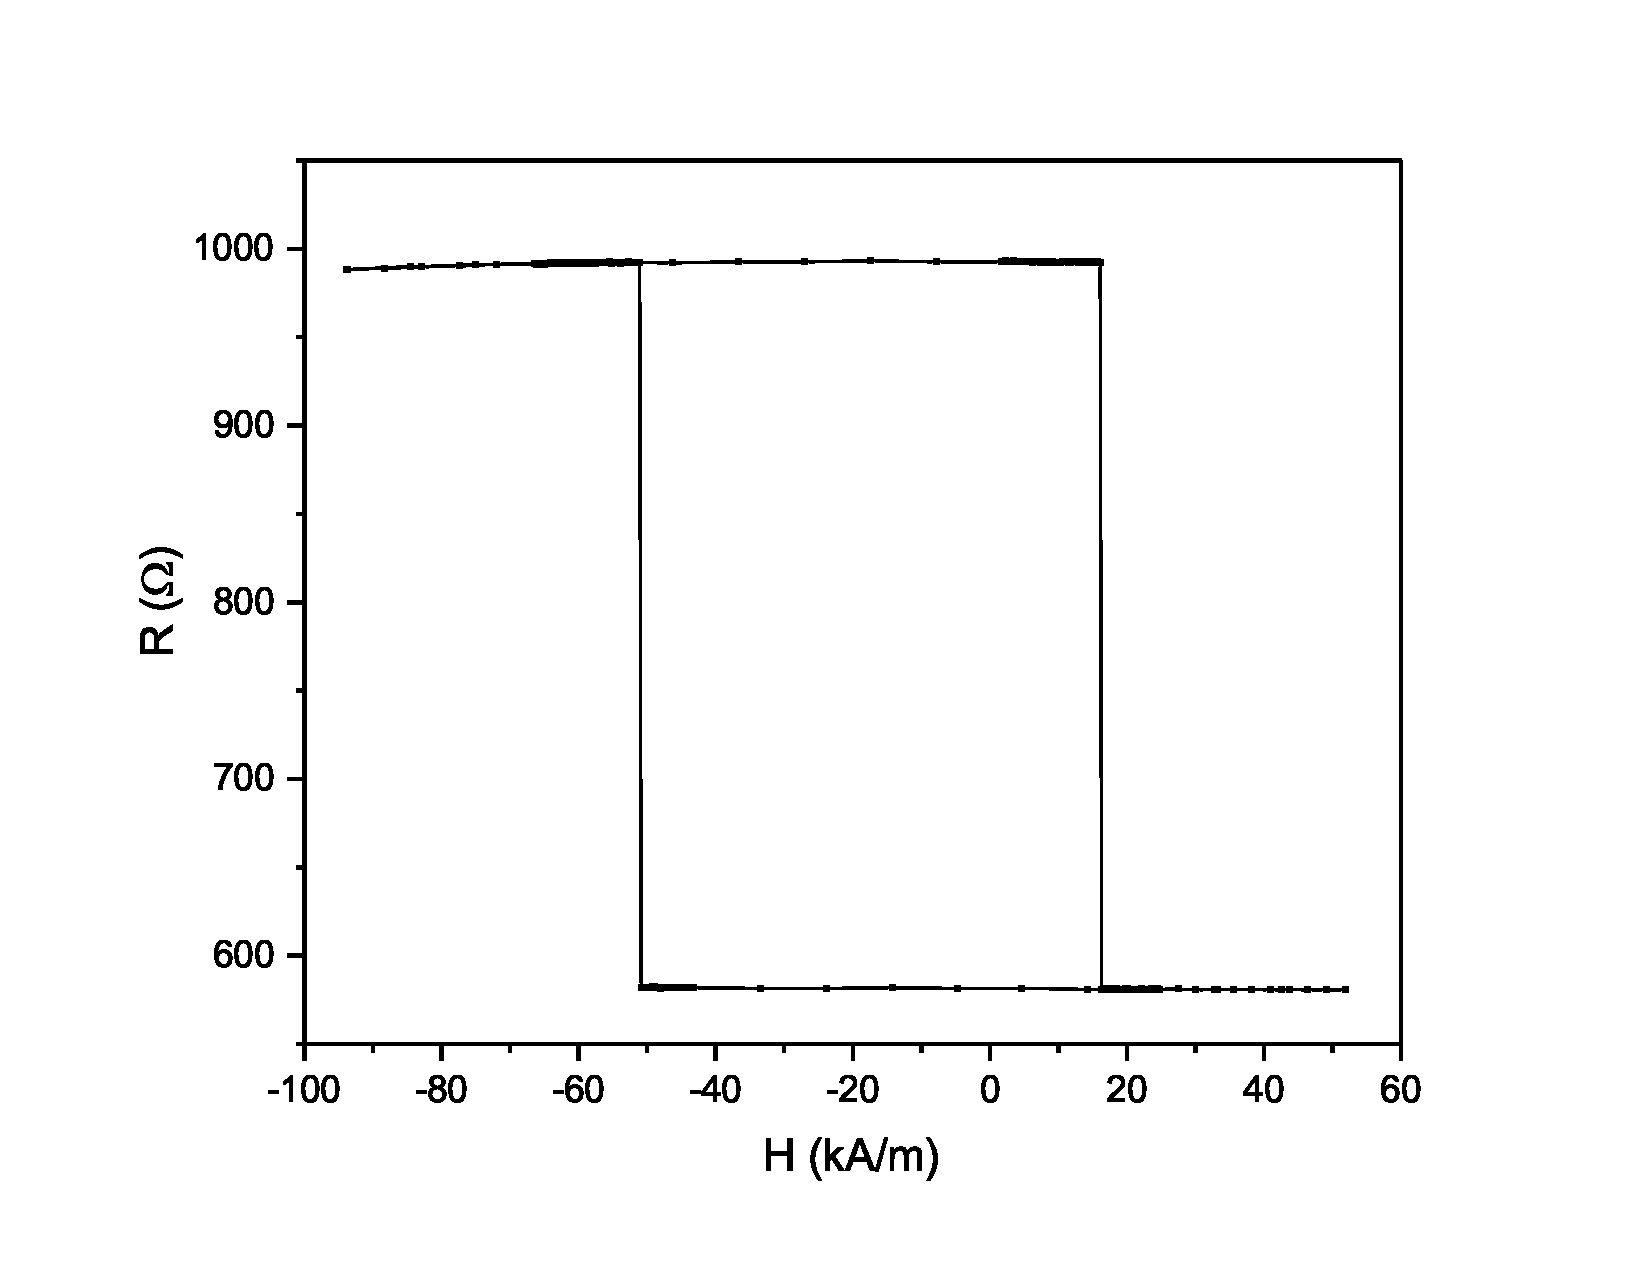
\includegraphics[width=0.75\paperwidth]{img/05/ResultsTMR.eps}
        \caption{Hysteresis loop measured for a single storage element (MTJ). Two stable states are observed for \SI[parse-numbers = false, number-math-rm = \ensuremath, per-mode=symbol]{H = 0}{\ampere\per\metre}. TMR is equal to \SI{70.6}{\percent}}
        \label{ExperimentMeasurementTMRSingle}
    \end{figure}
    
    \begin{figure}[H]
        \centering
        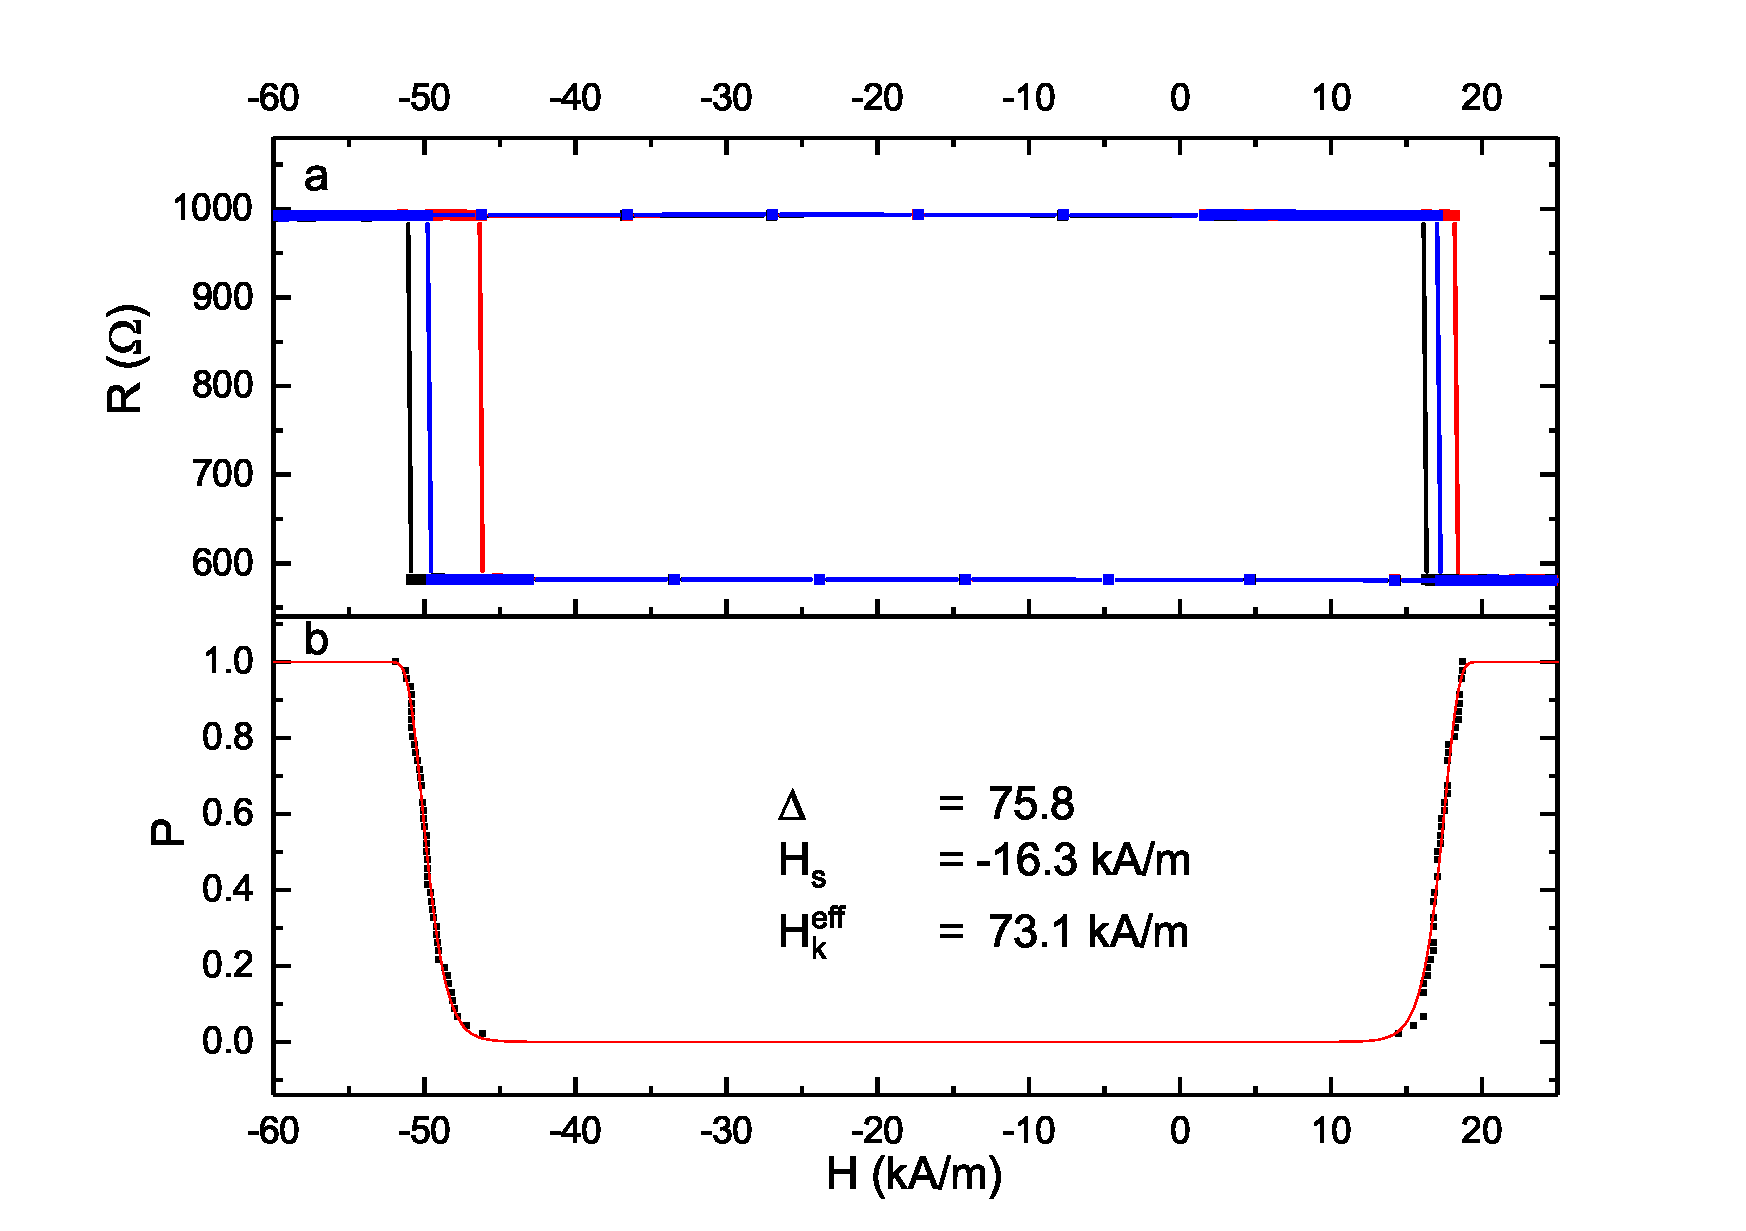
\includegraphics[width=0.65\paperwidth]{img/05/StabilitySato.eps}
        \caption{a) Representative TMR loops, with densified measurement points in regions where switching is expected to take place, b) calculated (based on measurements) switching probability (black points) and fitted theoretical curve. Derived $\Delta$, $H_s$ and $H_k^{eff}$ are presented. }
        \label{ExperimentMeasurementTMRSato}
    \end{figure}
    
    \begin{figure}[H]
        \centering
        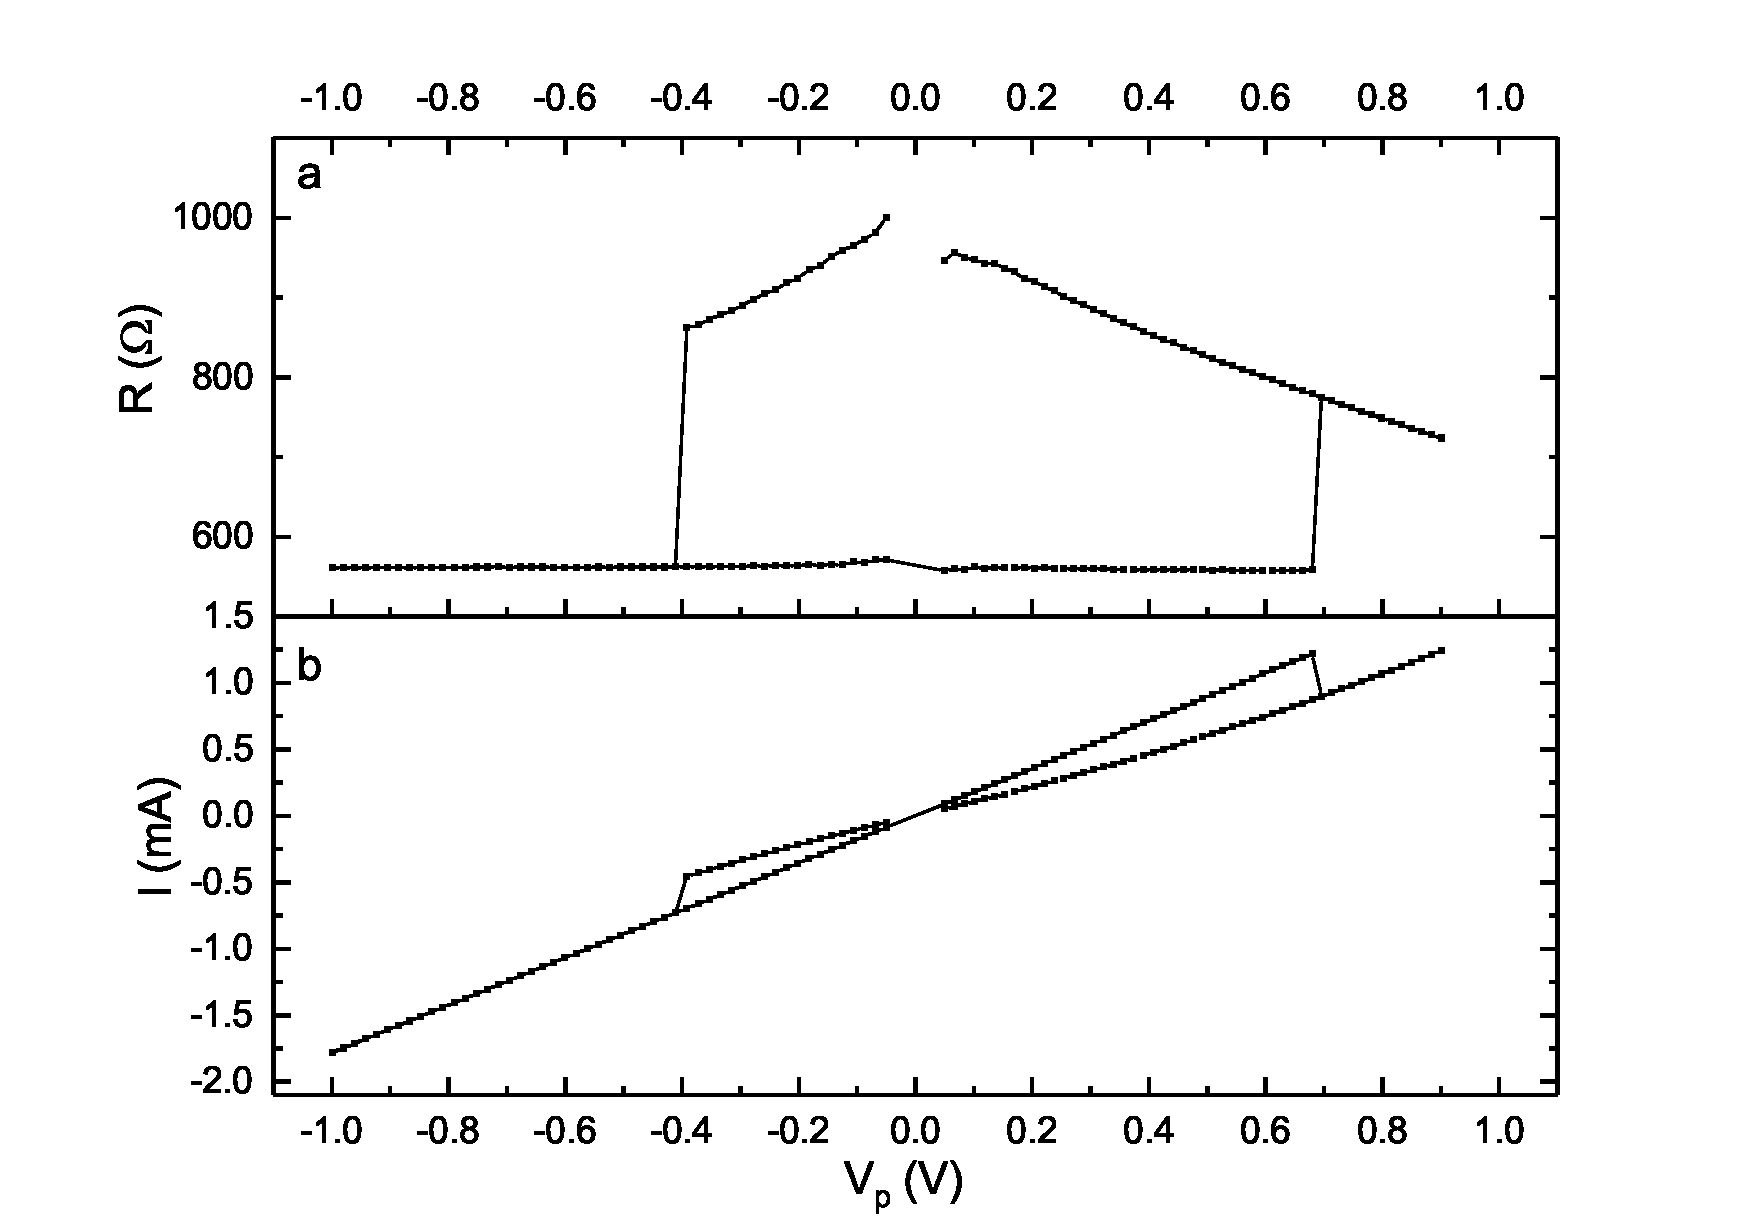
\includegraphics[width=0.65\paperwidth]{img/05/ResultsCIMS1.eps}
        \caption{Resistance (a) and current (b) versus $V_p$ at \SI[parse-numbers = false, number-math-rm = \ensuremath, per-mode=symbol]{H = 0}{\ampere\per\metre} for a single storage element. CIMS effect is observed.}
        \label{ExperimentMeasurementCIMS1}
    \end{figure}
    
    CIMS measurements (Fig. \ref{ExperimentMeasurementEye} a) were repeated with a range of external magnetic field $H$ applied. For each external magnetic field, switching voltages from P to AP and vice versa were established, and plotted as voltage versus magnetic field (Fig. \ref{ExperimentMeasurementEye} b). These points created a stability diagram, which shows the region, where both P and AP states are stable, as well as only one of them above and below the region. Going outside P/AP stability region (by changing magnetic field, or amplitude of the voltage pulse) results in changing state to P or AP (writing data), while remaining inside the area allows measuring the resistance of the element (reading the data).
    
    \begin{figure}[H]
        \centering
        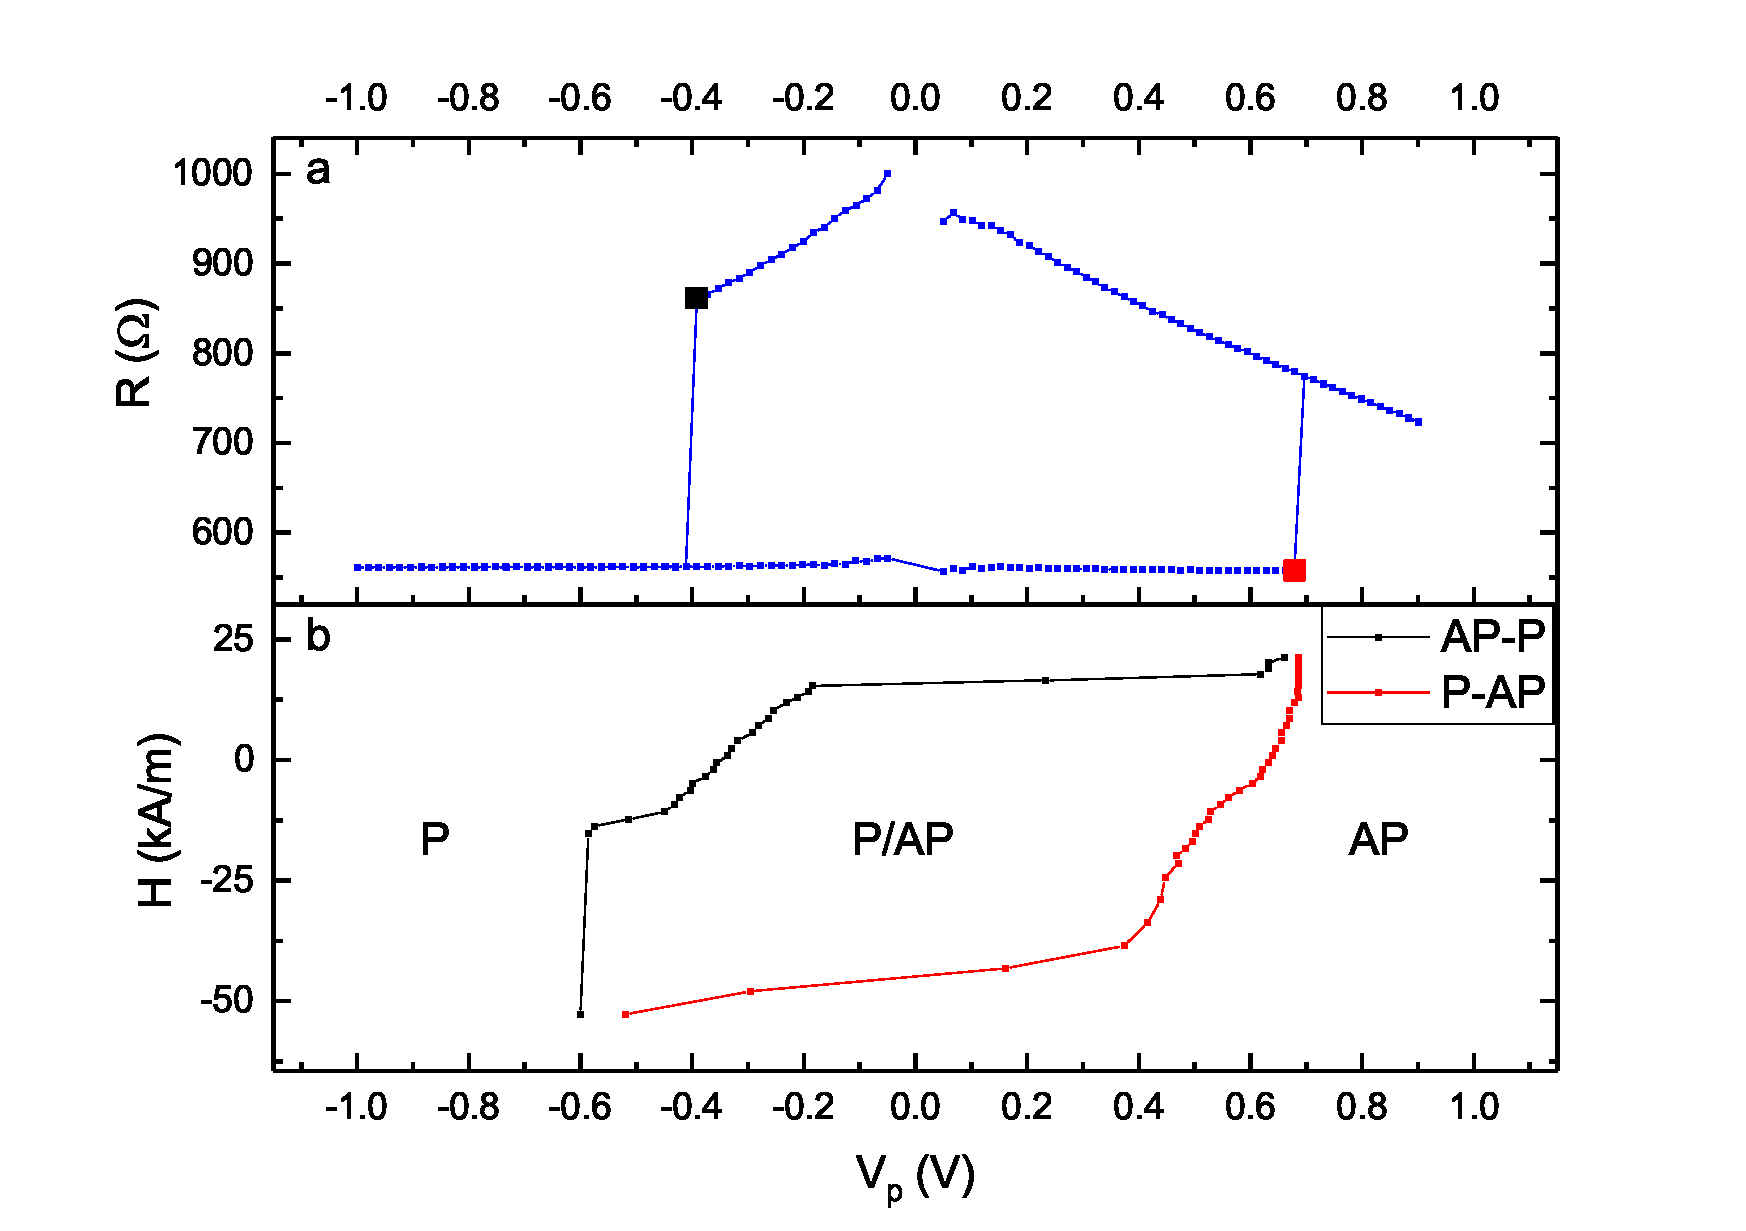
\includegraphics[width=0.7\paperwidth]{img/05/ResultsEye.eps}
        \caption{a) Representative CIMS measurement result at \SI[parse-numbers = false, number-math-rm = \ensuremath, per-mode=symbol]{H = 0}{\ampere\per\metre}. Switching from AP to P, and from P to AP marked with black and red symbol, respectively, b) Stability diagram of the storage element. Lines indicate switching from P to AP or vice versa. Regions are marked with possible states of the storage MTJ (P, P/AP, AP).}
        \label{ExperimentMeasurementEye}
    \end{figure}

    It is vital to notice, that the element in zero field can be stable in both P and AP states and, therefore, it can be used as non-volatile storage without external magnetic field.    
    
    Some of the elements on the sample were found not working (no connection or short-circuit) due to non-ideal fabrication process.
    
\subsection{Dual bit storage cell experiment} \label{sec:ExperimentMeasurementsDual}
    
    After the successful verification of operation of a single storage element, on a proper section of the sample three serially connected elements were selected and tested during CIMS measurements (Fig. \ref{ExperimentMeasurementCIMS2}). In subsequent measurements $V_{pos}$ was increased. The predicted behaviour (Fig. \ref{PrinciplesSeriesCIMS}) of serially connected storage elements was confirmed. In such storage cell, constructed of three individual storage elements, four stable states can be defined, and binary numbers can be assigned to them: 
    
    \begin{itemize}[noitemsep,label=\textbullet]
    	\item all elements in AP state $\Longrightarrow$ "11"
    	\item one element in P state and two elements in AP state $\Longrightarrow$ "10"
    	\item two elements in P state and one element in AP state $\Longrightarrow$ "01"
    	\item all elements in P state $\Longrightarrow$ "00"
    \end{itemize}
    
    Also, voltages to write particular states, as well as a region safe for reading the storage cell can be defined (Fig. \ref{ExperimentMeasurementCIMS2} a). 
    
    \begin{figure}[H]
        \centering
        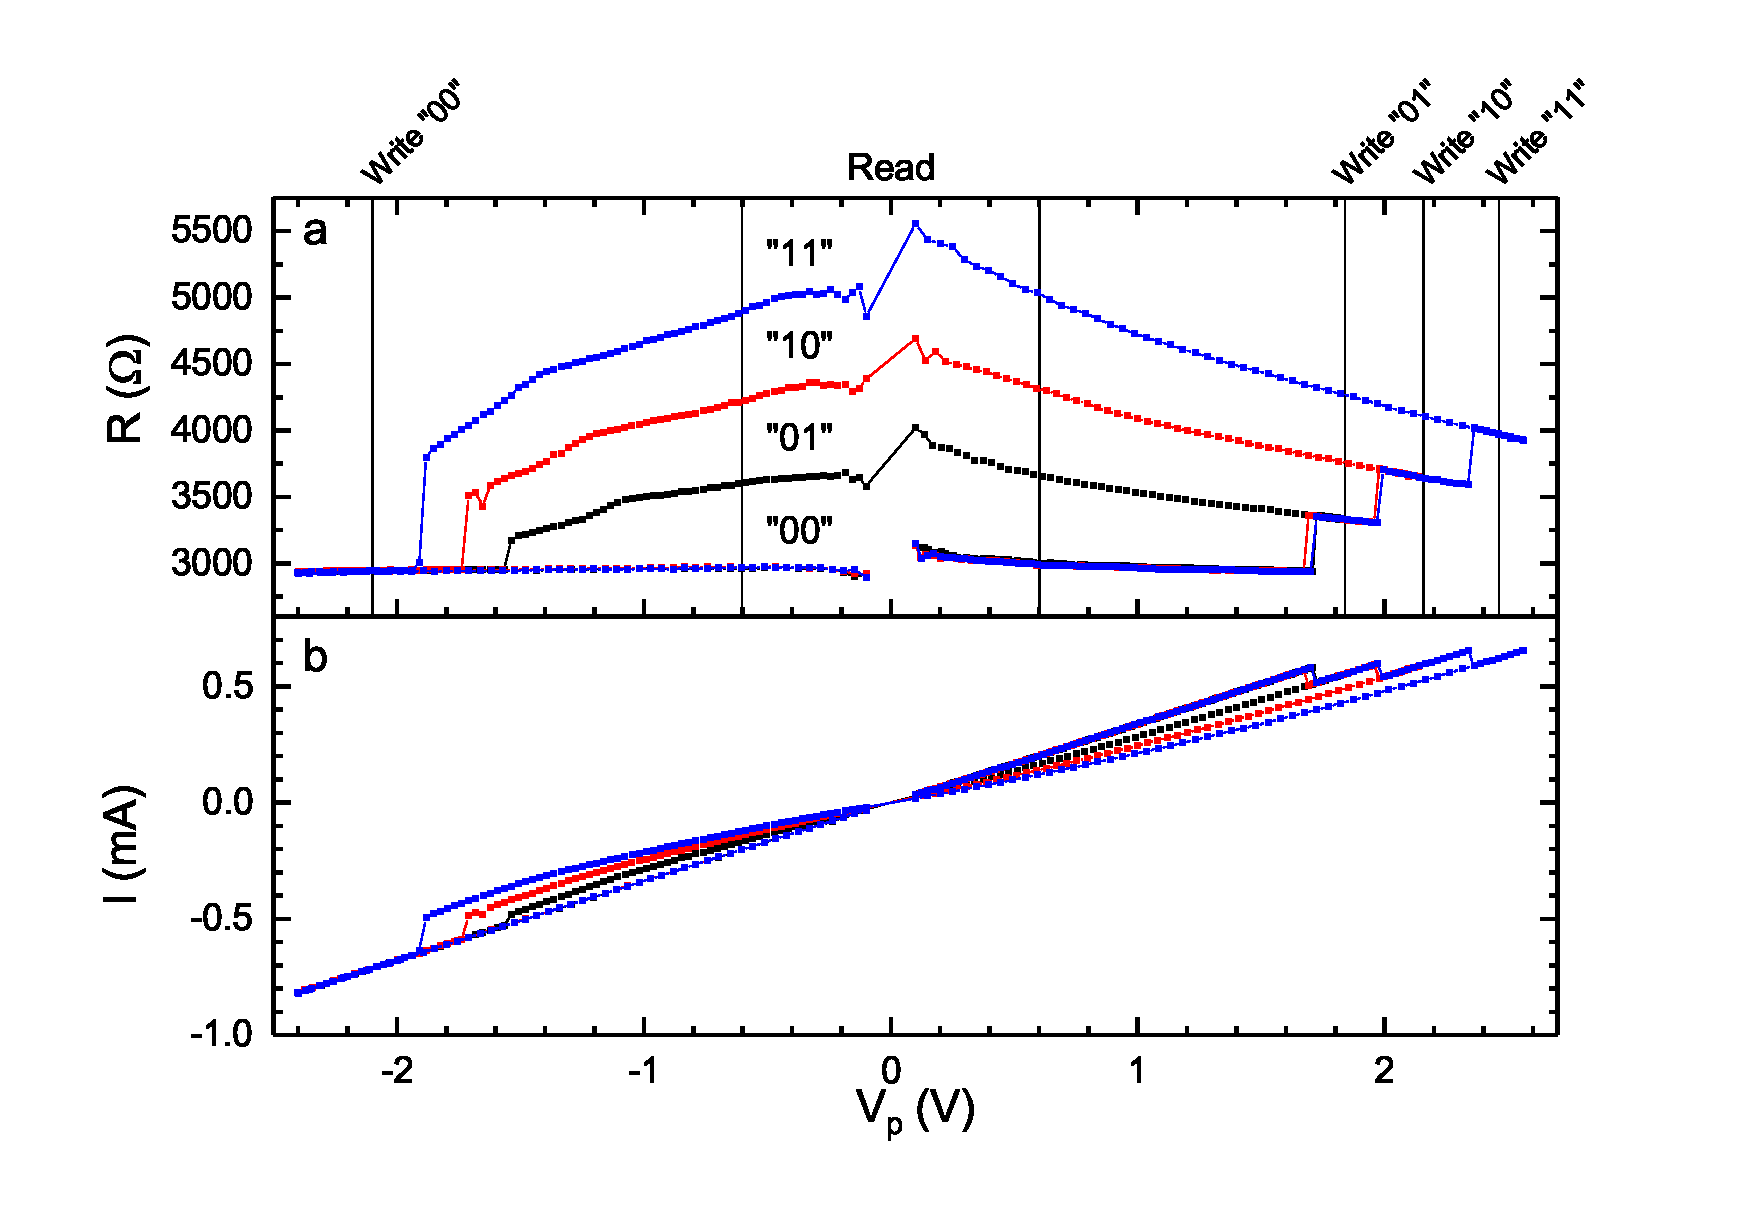
\includegraphics[width=0.7\paperwidth]{img/05/ResultsCIMS2.eps}
        \caption{Results of CIMS measurement for storage cell constructed of three serially connected storage elements. Resistance changes for loops measured with different $V_{pos}$ (different colours) prove the ability of the storage cell to act as a multi-bit cell. The proposed binary coding, voltages for writing, and safe readout are presented (a). Current changes during the process (b).}
        \label{ExperimentMeasurementCIMS2}
    \end{figure}
    
    Also, the principle of operation, involving the current decreasing below the critical current after one element switching into AP state, was confirmed (Fig. \ref{ExperimentMeasurementCIMS2Zoom}). Due to non-ideal manufacturing process, critical currents of all incorporated elements are non-equal, but this has no adverse effect on the process.
    
    \begin{figure}[H]
        \centering
        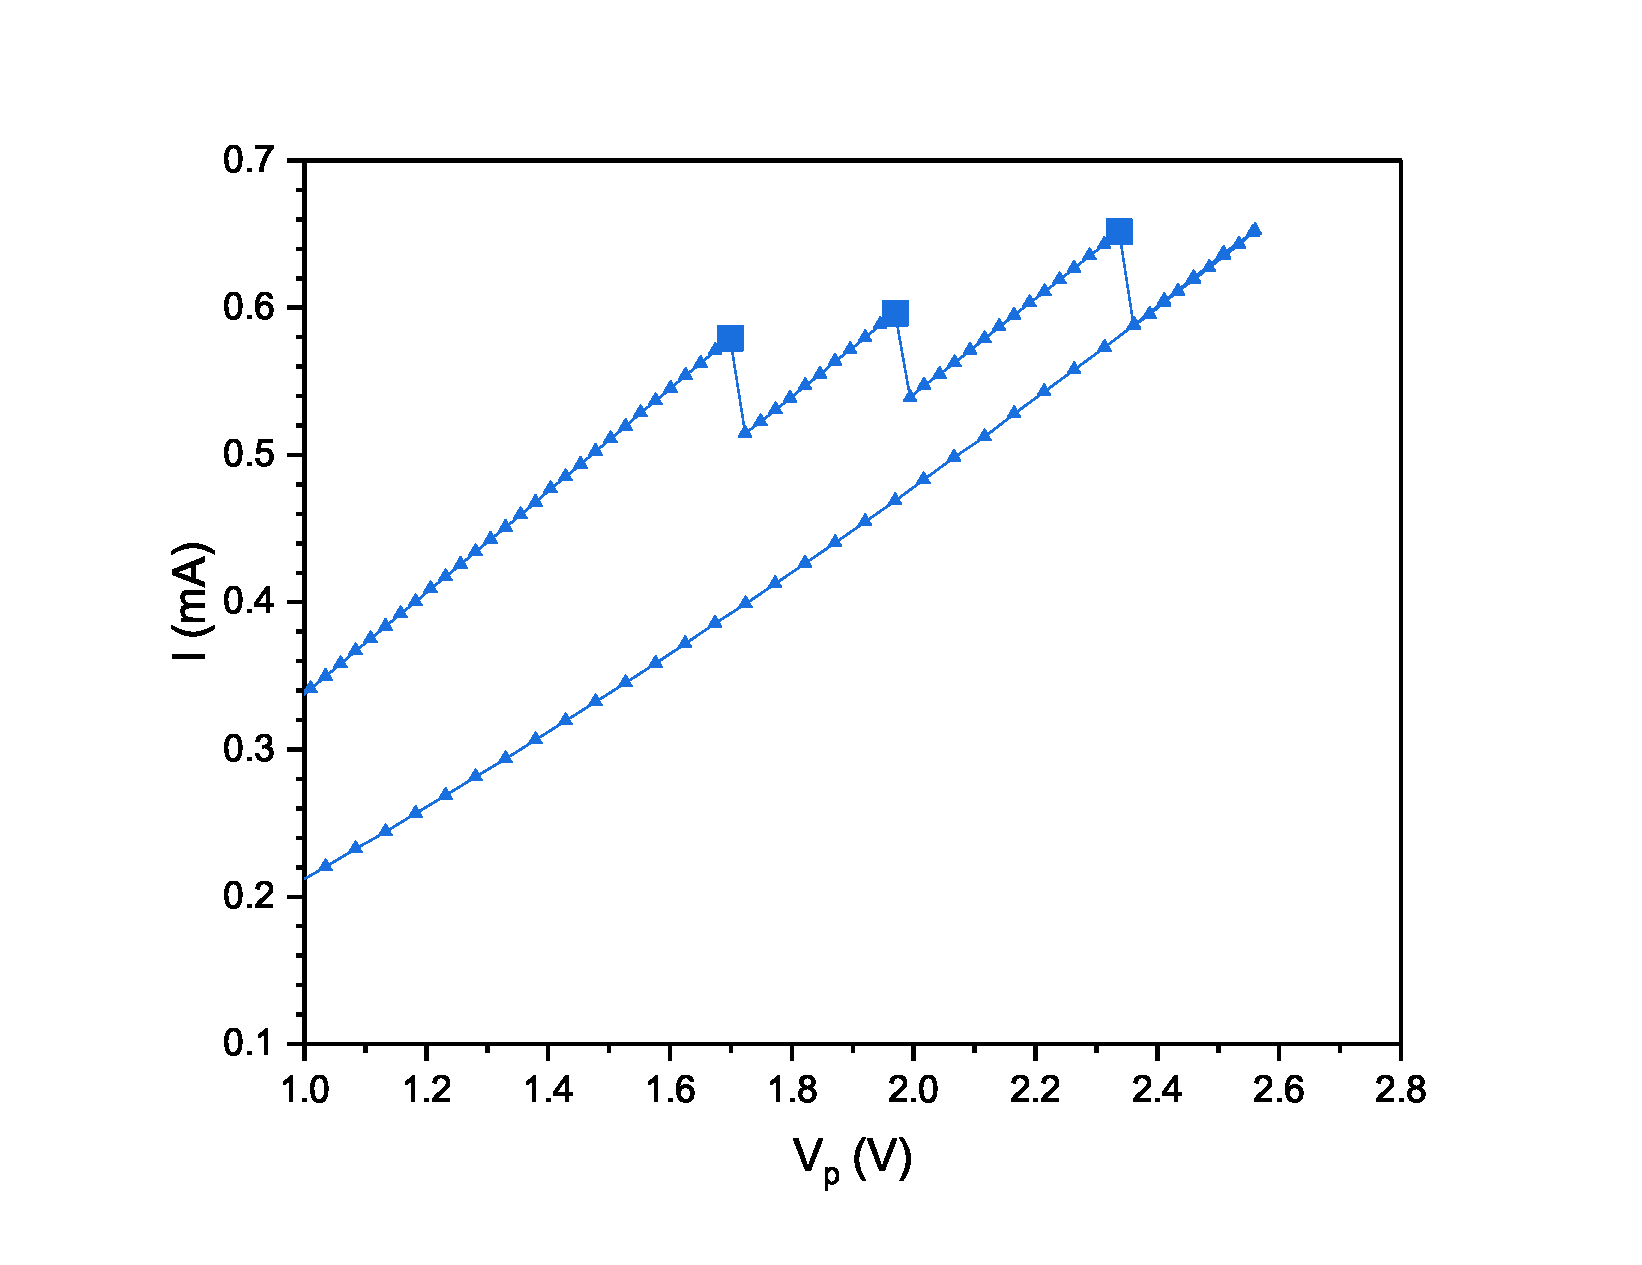
\includegraphics[width=0.7\paperwidth]{img/05/ResultsCIMS2Zoom.eps}
        \caption{A close up of current in the CIMS measurement. Critical currents, causing subsequent elements to switch to the AP state are marked with squares.}
        \label{ExperimentMeasurementCIMS2Zoom}
    \end{figure}

\subsection{Triple bit storage cell experiment} \label{sec:ExperimentMeasurementsTripple}    
    
    Utilising the mechanism a storage cell constructed of seven storage elements were subjected to CIMS measurement. As predicted, the cell exhibited eight stable states (Fig. \ref{ExperimentMeasurementCIMS3}). The issue was noticed, that regions for writing some of the states are very narrow, due to variation of the switching voltage (related with the switching current). It is believed, that the behaviour is due to very similar critical currents of all incorporated elements. Also switching to "000" state was not ideal in the case, and needs further investigation.
    
    \begin{figure}[H]
        \centering
        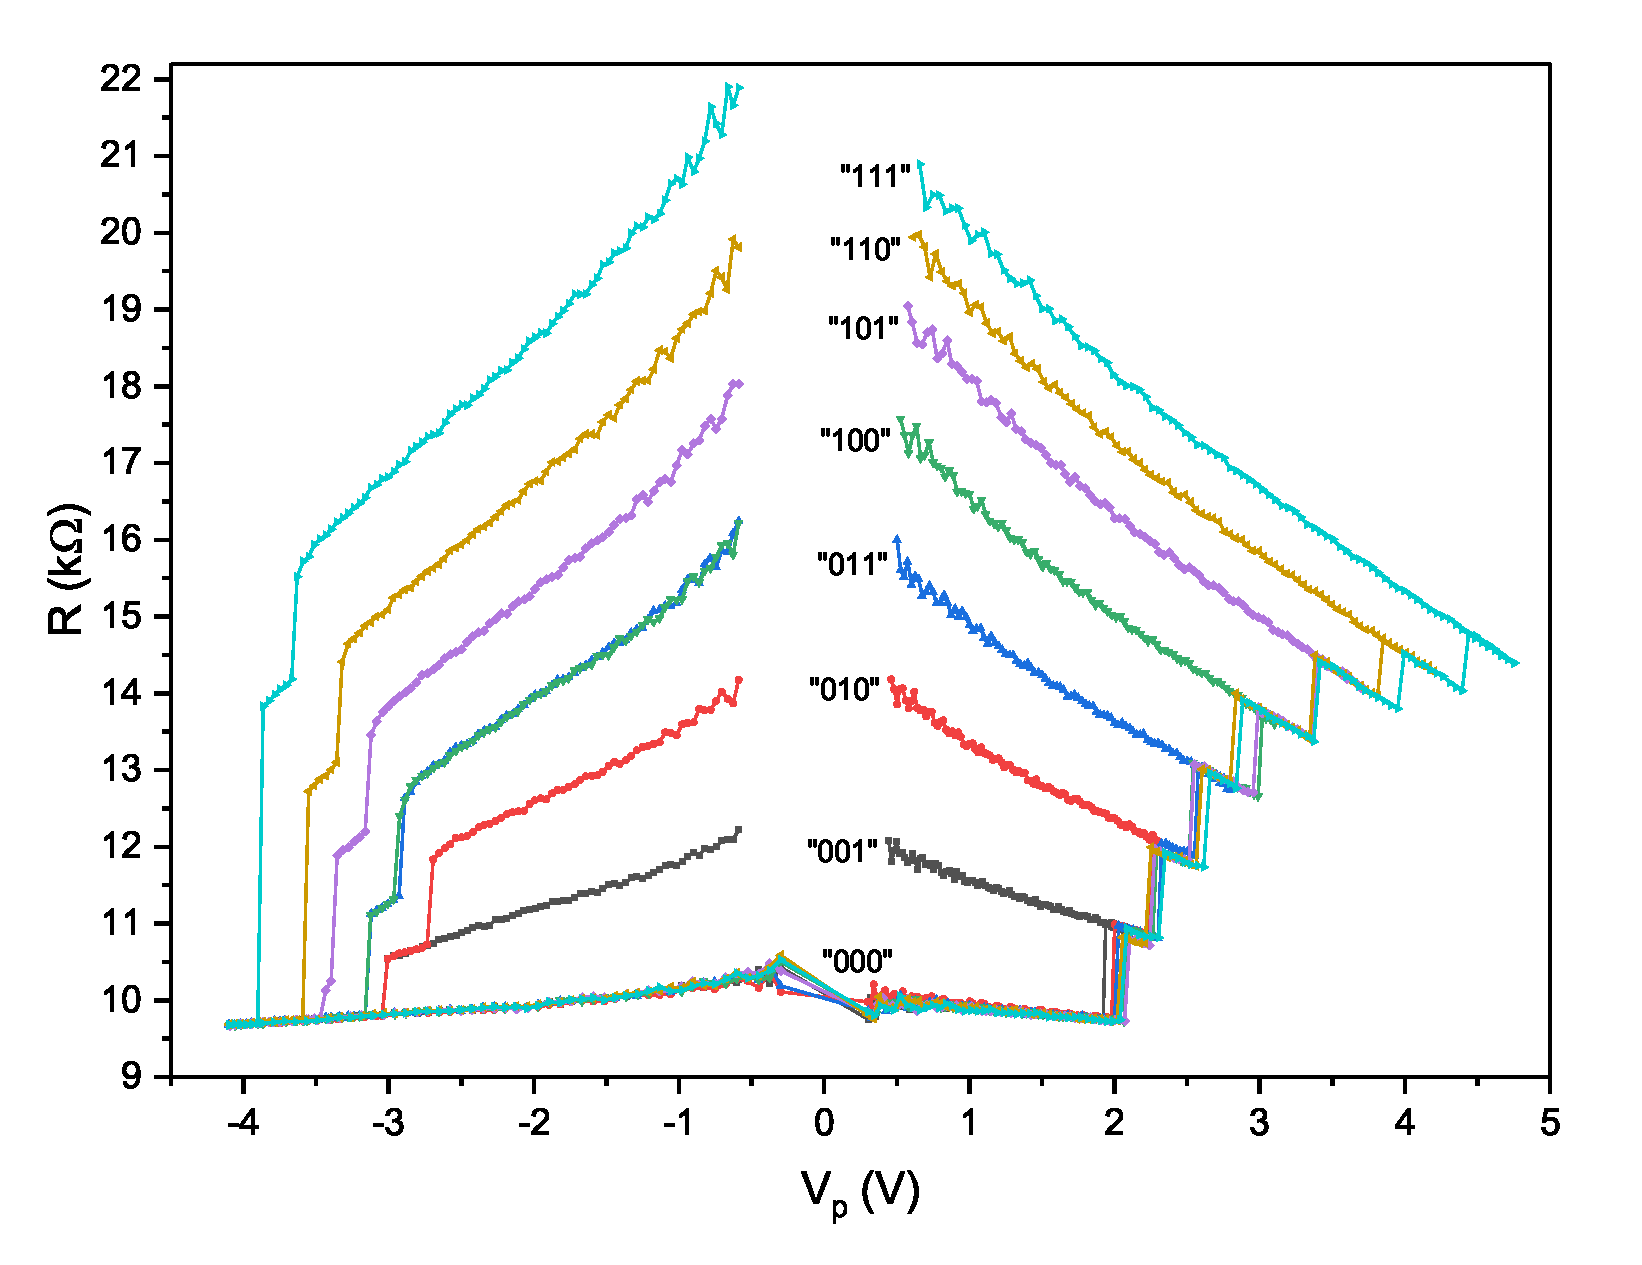
\includegraphics[width=0.7\paperwidth]{img/05/ResultsCIMS3.eps}
        \caption{Results of CIMS measurement for storage cell constructed of seven serially connected storage elements. Resistance changes for loops measured with different $V_{pos}$ are presented in different colours. The proposed binary coding is presented.}
        \label{ExperimentMeasurementCIMS3}
    \end{figure}

\section{Experiment summary} \label{sec:ExperimentSummary}

    The conducted experiments were successful and confirmed the predicted behaviour of single storage elements as well as multi-bit (two- and three-bit) storage cells. Larger cells were not tested, because it was not possible to find 15 subsequent serially connected working storage elements and also miniaturised storage cells were not operating due to fabrication issues.